\documentclass[10pt]{article}

%%%%%%%%%%%%%%%%%%%%%%%%%%%%%%%%%%%%%%%%%%%%%%%%%%%%%%%%%%%%%%%%%%%%%%%%%%%%%%%%
% LaTeX Imports
%%%%%%%%%%%%%%%%%%%%%%%%%%%%%%%%%%%%%%%%%%%%%%%%%%%%%%%%%%%%%%%%%%%%%%%%%%%%%%%%
\usepackage{amsfonts}                                                   % Math fonts
\usepackage{amsmath}                                                    % Math formatting
\usepackage{amssymb}                                                    % Math formatting
\usepackage{amsthm}                                                     % Math Theorems
\usepackage{arydshln}                                                   % Dashed hlines
\usepackage{attachfile}                                                 % AttachFiles
\usepackage{cancel}                                                     % Cancelled math
\usepackage{caption}                                                    % Figure captioning
\usepackage{color}                                                      % Nice Colors
\input{./lib/dragon.inp}                                                % Tikz dragon curve
\usepackage[ampersand]{easylist}                                        % Easy lists
\usepackage{fancyhdr}                                                   % Fancy Header
\usepackage[T1]{fontenc}                                                % Specific font-encoding
%\usepackage[margin=1in, marginparwidth=2cm, marginparsep=2cm]{geometry} % Margins
\usepackage{graphicx}                                                   % Include images
\usepackage{hyperref}                                                   % Referencing
\usepackage[none]{hyphenat}                                             % Don't allow hyphenation
\usepackage{lipsum}                                                     % Lorem Ipsum Dummy Text
\usepackage{listings}                                                   % Code display
\usepackage{marginnote}                                                 % Notes in the margin
\usepackage{microtype}                                                  % Niceness
\usepackage{lib/minted}                                                 % Code display
\usepackage{multirow}                                                   % Multirow tables
\usepackage{pdfpages}                                                   % Include pdfs
\usepackage{pgfplots}                                                   % Create Pictures
\usepackage{rotating}                                                   % Figure rotation
\usepackage{setspace}                                                   % Allow double spacing
\usepackage{subcaption}                                                 % Figure captioning
\usepackage{tikz}                                                       % Create Pictures
\usepackage{tocloft}                                                    % List of Equations
%%%%%%%%%%%%%%%%%%%%%%%%%%%%%%%%%%%%%%%%%%%%%%%%%%%%%%%%%%%%%%%%%%%%%%%%%%%%%%%%
% Package Setup
%%%%%%%%%%%%%%%%%%%%%%%%%%%%%%%%%%%%%%%%%%%%%%%%%%%%%%%%%%%%%%%%%%%%%%%%%%%%%%%%
\hypersetup{%                                                           % Setup linking
    colorlinks=true,
    linkcolor=black,
    citecolor=black,
    filecolor=black,
    urlcolor=black,
}
\RequirePackage[l2tabu, orthodox]{nag}                                  % Nag about bad syntax
\renewcommand*\thesection{\arabic{section} }                             % Reset numbering
\renewcommand{\theFancyVerbLine}{ {\arabic{FancyVerbLine} } }              % Needed for code display
\renewcommand{\footrulewidth}{0.4pt}                                    % Footer hline
\setcounter{secnumdepth}{3}                                             % Include subsubsections in numbering
\setcounter{tocdepth}{3}                                                % Include subsubsections in toc
%%%%%%%%%%%%%%%%%%%%%%%%%%%%%%%%%%%%%%%%%%%%%%%%%%%%%%%%%%%%%%%%%%%%%%%%%%%%%%%%
% Custom commands
%%%%%%%%%%%%%%%%%%%%%%%%%%%%%%%%%%%%%%%%%%%%%%%%%%%%%%%%%%%%%%%%%%%%%%%%%%%%%%%%
\newcommand{\nvec}[1]{\left\langle #1 \right\rangle}                    %  Easy to use vector
\newcommand{\ma}[0]{\mathbf{A} }                                         %  Easy to use vector
\newcommand{\mb}[0]{\mathbf{B} }                                         %  Easy to use vector
\newcommand{\abs}[1]{\left\lvert #1 \right\rvert}                       %  Easy to use abs
\newcommand{\pren}[1]{\left( #1 \right)}                                %  Big parens
\let\oldvec\vec
\renewcommand{\vec}[1]{\oldvec{\mathbf{#1} } }                            %  Vector Styling
\newtheorem{thm}{Theorem}                                               %  Define the theorem name
\newtheorem{definition}{Definition}                                     %  Define the definition name
\definecolor{bg}{rgb}{0.95,0.95,0.95}
\newcommand{\java}[4]{\vspace{10pt}\inputminted[firstline=#2,
                                 lastline=#3,
                                 firstnumber=#2,
                                 gobble=#4,
                                 frame=single,
                                 label=#1,
                                 bgcolor=bg,
                                 linenos]{java}{#1} }
\newcommand{\python}[4]{\vspace{10pt}\inputminted[firstline=#2,
                                 lastline=#3,
                                 firstnumber=#2,
                                 gobble=#4,
                                 frame=single,
                                 label=#1,
                                 bgcolor=bg,
                                 linenos]{python}{#1} }
\newcommand{\js}[4]{\vspace{10pt}\inputminted[firstline=#2,
                                 lastline=#3,
                                 firstnumber=#2,
                                 gobble=#4,
                                 frame=single,
                                 label=#1,
                                 bgcolor=bg,
                                 linenos]{js}{#1} }
%%%%%%%%%%%%%%%%%%%%%%%%%%%%%%%%%%%%%%%%%%%%%%%%%%%%%%%%%%%%%%%%%%%%%%%%%%%%%%%%
% Beginning of document items - headers, title, toc, etc...
%%%%%%%%%%%%%%%%%%%%%%%%%%%%%%%%%%%%%%%%%%%%%%%%%%%%%%%%%%%%%%%%%%%%%%%%%%%%%%%%
\pagestyle{fancy}                                                       %  Establishes that the headers will be defined
\fancyhead[LE,LO]{Computer Systems Notes}                                  %  Adds header to left
\fancyhead[RE,RO]{Zoe Farmer}                                       %  Adds header to right
\cfoot{ \thepage }
\lfoot{CSCI 2400}
\rfoot{Han}
\title{Computer Systems Notes}
\author{Zoe Farmer}

%%%%%%%%%%%%%%%%%%%%%%%%%%%%%%%%%%%%%%%%%%%%%%%%%%%%%%%%%%%%%%%%%%%%%%%%%%%%%%%%
% Beginning of document items - headers, title, toc, etc...
%%%%%%%%%%%%%%%%%%%%%%%%%%%%%%%%%%%%%%%%%%%%%%%%%%%%%%%%%%%%%%%%%%%%%%%%%%%%%%%%
\pagestyle{fancy}                                                 %  Establishes that the headers will be defined
\fancyhead[LE,LO]{Problem Set 7}                                  %  Adds header to left
\fancyhead[RE,RO]{Zoe Farmer, Jeremy Granger, Ryan Roden}     %  Adds header to right
\cfoot{\mlptikz[size=0.25in, text=on, textposx=0, textposy=0, textvalue=\thepage, textscale=0.75in]{applejack}}
\lfoot{CSCI 3104}
\rfoot{Clauset}
\title{Problem Set Seven}
\author{Zoe Farmer\\Jeremy Granger\\Ryan Roden}
%%%%%%%%%%%%%%%%%%%%%%%%%%%%%%%%%%%%%%%%%%%%%%%%%%%%%%%%%%%%%%%%%%%%%%%%%%%%%%%%
% Beginning of document items - headers, title, toc, etc...
%%%%%%%%%%%%%%%%%%%%%%%%%%%%%%%%%%%%%%%%%%%%%%%%%%%%%%%%%%%%%%%%%%%%%%%%%%%%%%%%
\begin{document}

\maketitle

\begin{easylist}[enumerate]
    @ Professor Dumbledore needs your help to compute the in and out degrees of all vertices in a directed multigraph
    $G$. However, he is not sure how to represent the graph so that the calculation is most efficient. For each of the
    three possible representations, express your answers in asymptotic notation (the only notation Dumbledore
    understands), in terms of $V$ and $E$, and justify your claim.
    @@ An edge list representation. Assume vertex indices can be arbitrary.
    @@@ The asymptotic complexity of this is $O(|E|)$  because it iterates over all edges of each node for endpoints
    between vertices adding to the in and out-degree hash tables as it goes. We know that adding to a hash table is
    approximately constant time, so our total time is $O(|E|) + O(1) = O(|E|)$.
    @@ An adjacency list representation. Assume the vector's length is known.
    @@@ The asymptotic complexity of this is $O(|V| + |E|)$ because we need to iterate through each node in the
    adjacency list and each edge associated with each node, adding to a hash table tabulating the degrees as we go. The
    out degree of any given node is the length of its edge list, while the in degree is calculated as the edges are
    iterated over by adding to each edge endpoint's in degree.
    @@ An adjacency matrix representation. Assume the size of the matrix is known.
    @@@ This is the easiest to determine, as the in degree of any node is simply the sum of the corresponding column in
    the array, while its out degree is the sum of its row. A sum operation is $O(|V|)$, therefore the total complexity
    is $2 O(|V|^2)$.

    @ Let $G = (E, V)$ denote a directed multigraph. A simple and undirected graph is a $G = (V, E)$, such that
    $E^\prime$ is derived from the edges in $E$ so that (i) every directed multi-edge, e.g., $\{(u, v), (u, v)\}$ or
    even simply $\{(u, v)\}$, has been replaced by a single pair of directed edges $\{(u, v), (v, u)\}$ and (ii) all
    self-loops $(u, u)$ have been removed.\newline

    Describe and analyze an algorithm (explain how it works, give pseudocode if necessary, derive its running time and
    space usage, and prove its correctness) that takes time $O(V + E)$ and $O(E)$ space to convert $G$ into $G^\prime$.
    Assume both $G$ and $G^\prime$ are stored as adjacency lists.

    @@ First replace every edge list with a hash table. Then iterate through the adjacency list, letting the current
    node be denoted by $i$. For every node $i$ with edge list consisting of edges denoted by $j$, insert $i$ into $j$'s
    hash table. If any $i$ is found in $j$, ignore it. After iterating through the nodes, convert each edge hash back
    into an edge list. \newline

    As the iteration occurs, any repeat instance of the $i$th node will be ignored, and not added to our hash tables,
    which in essence removes them. Any edge will also be added to the destination node's edge hash table, which when we
    convert back to an array by indexing by keys we obtain our non-duplicating edge lists.\newline
    
    When our algorithm iterates, we are visiting every node, regardless of its loop-connection relations.  Because of
    this, we are guaranteed O(V) time. During our steps through the adjacency list, we are inspecting each node's edge
    list.  We are converting our directed edges to undirected edges (by essentially adding a new node-edge relationship)
    which is a constant time operation.  Because each edge is compared within our adjacency list, we must add O(E) time.
    Thus, the total running time approaches O(V + E) asymptotically.

    @ A graph $(V, E)$ is bipartite iff the vertices $V$ can be partitioned into two subsets $L$ and $R$, such that
    every edge has one end in $L$ and the other in $R$.
    @@ Prove that every tree is a bipartite graph.
    @@@ Given our input tree $T_0$ with two branches $L_0$ and $R_0$, we can see that by definition of a tree no node in
    $L_0$ can connect to any node in $R_0$. This means that each level can be thought of as a different ``side'' of the
    bipartite graph. To prove this consider the graph coloring problem. Start by coloring the root node, $T_0$ red, and
    it's children ($R_0, L_0$) blue. Recursively apply this operation with color red and blue alternating as you go. At
    the bottom of the tree every level will be either red or blue, with no node in a single colored level connecting to
    another node. If at any point we have an odd-length cycle the definition of a tree will no longer hold, and the
    graph can no longer be bipartite.
    @@ Adapt an algorithm described in class so that it will determine whether a given undirected graph is bipartite.
    Give and justify its running time.
    @@@ The runtime of the below algorithm is $O(|V| + |E|)$, since we are using an adaptation of the previously
    discussed {\ttfamily Search-Tree} function.  The algorithm starts assuming that all nodes are clean and that their
    color is set to "None."  It then steps into the tree and sets the root node to red.  From there, the first child is
    set to blue and the second child is red.  The graph is traversed using this standard and the connected nodes are
    compared.  If at any time they are the same color, We conclude that the graph is not bipartite.  The process of
    visiting every node in the tree and assigning a color takes O(V) time because there are V total nodes.
    Additionally, since every edge relationship is also visited to determine whether any connected nodes are the same
    color, we must add O(E) time because there are E edges.  Thus, total asymptotic time of this algorithm is O(V + E).  

    \begin{lstlisting}
        def search_tree(nodes, s):
            # Input: Adjacency list graph structure
            #        [('a', [1, 2, ..., n0]),
            #         ('b', [1, 2, ..., n1]),
            #         :
            #         ('m', [1, 2, ..., nm])]
            # Where this list is a list of tuples with node name, and a
            # list of indices that it points to.
            size = len(nodes)
            v    = [0 for i in range(size)]
            d    = [-1 for i in range(size)]
            c    = [None for i in range(size)]
            q    = [s]
            d[s] = 0
            while len(q) > 0:
                x = q.pop()
                if v[x] == 0:
                    if c[x] is None and p[x] is None:
                        c[x] = 'red'
                    elif c[x] is None:
                        c[x] = 'blue'
                        if c[p[x]] is 'blue':
                            c[x] = 'red'
                    for y in nodes[x][1]:
                        if v[y] == 0:
                            q.append(y)
                            d[y] = d[x] + 1
                    v[x] = 1
            flag = True
            for node in range(size):
                edges = nodes[node][1]
                for j in range(len(edges)):
                    edge = edges[j]
                    if c[node] == c[edge]:
                        flag = False
            return flag
    \end{lstlisting}

    @ Professor Snape tells you that when an adjacency matrix representation is used, most graph algorithms take
    $\Omega(|V|^2)$ time, but there are some exceptions. Snape claims that determining whether a directed graph $G$
    contains a universal sink, which is defined as a vertex with in-degree $|V| - 1$ (i.e., every other vertex points to
    this one) and out-degree 0, can be done in time $O(|V|)$, given an adjacency matrix for $G$. Show that Snape is
    correct.
    @@ The below algorithm will determine whether or not a universal sink exists for any given graph. It does this by
    exhaustively eliminating nodes that do not fit the given criteria, but never eliminating a sink if it exists. This
    is based on the properties of adjacency matrices with universal sinks.\newline
    
    Any adjacency matrix with a universal sink in position $i$ will have a column of all ones in the $i$th column save when $i == j$, and all zeros in the $i$th row. This means that whenever a one is found we can eliminate that row's corresponding node as a possible sink, while if a zero is found we can eliminate the corresponding column as a possible sink, noting that for if $i == j$ a zero is non-conclusive. Since we iterate over every column in our matrix, we will eliminate all invalid column nodes, and by dynamically adjusting $i$ as we run into more invalid nodes we also exhaustively find all invalid nodes.
    
    \begin{lstlisting}
        def sink(G):
            not_sinks = []
            i = 0
            for j in range(len(G)):
                element = G[i][j]
                if i == j and element == 1:
                    not_sinks.append(i)
                    i = j
                elif element == 0:
                    not_sinks.append(j)
                elif element == 1:
                    not_sinks.append(i)
                    i = j
            sink = node not in not_sinks
            if sink is None
                return False
            return True
    \end{lstlisting}

    @ Implement an efficient algorithm that computes the diameter of an unweighted, undirected input graph $G = (V, E)$,
    when $G$ is given in adjacency list format, and which takes $O(V + E)$ additional space. Write a paragraph
    explaining the algorithm, its running time, and how it satisfies the space requirement.
    @@ This algorithm is a derivation from the search-tree algorithm discussed in class, and will perform a
    breadth-first-search between every pair of nodes in order to identify the longest shortest path, which is by
    definition the diameter. The largest difference between the discussed search tree and this one is that when the
    below algorithm identifies the node it's been searching for it stop and returns the distance. The only storage
    needed for this algorithm to perform is the adjacency matrix representation (which has space $O(|V| + |E|)$, and 3
    arrays (with size $O(|V|)$, therefore the algorithm has a $O(|V| + |E|)$ space requirement.

    @ Use your implementation from 5 to conduct the following numerical experiment to produce three nice-looking
    figures.
    @@ For $c = 5$, show numerically that the expected diameter of $G(n, p)$ increases like $O(\log n)$. Because $G(n,
    p)$ is a random variable, you should average the diameter at a given value of $n$ over several independent
    realizations (e.g., > 10) to get as smooth a curve as you can. Don't forget to vary $n$ over a broad range. (One
    figure.) Include a paragraph the summarizes how you conducted the experiment.
    @@@ In order to complete this, we established a wrapper for our diameter function that for any given number of nodes
    runs 10 experiments and takes the mean values as a data point. We have 5 different datum to keep track of, the
    number of nodes, the diameter of the network, the realtime duration, the number of operations, and the amount of
    space required, which are all averaged and appended to our csv file. If you'll note in the above definition of our
    diameter algorithm each class instance records its space requirements and how many operations are required.

    We now use {\ttfamily R}'s {\ttfamily ggplot2} to graph the relationships.

    Which results in Figure (1).

    \begin{figure}[ht]
        \centering
        \begin{subfigure}[b]{0.48\textwidth}
            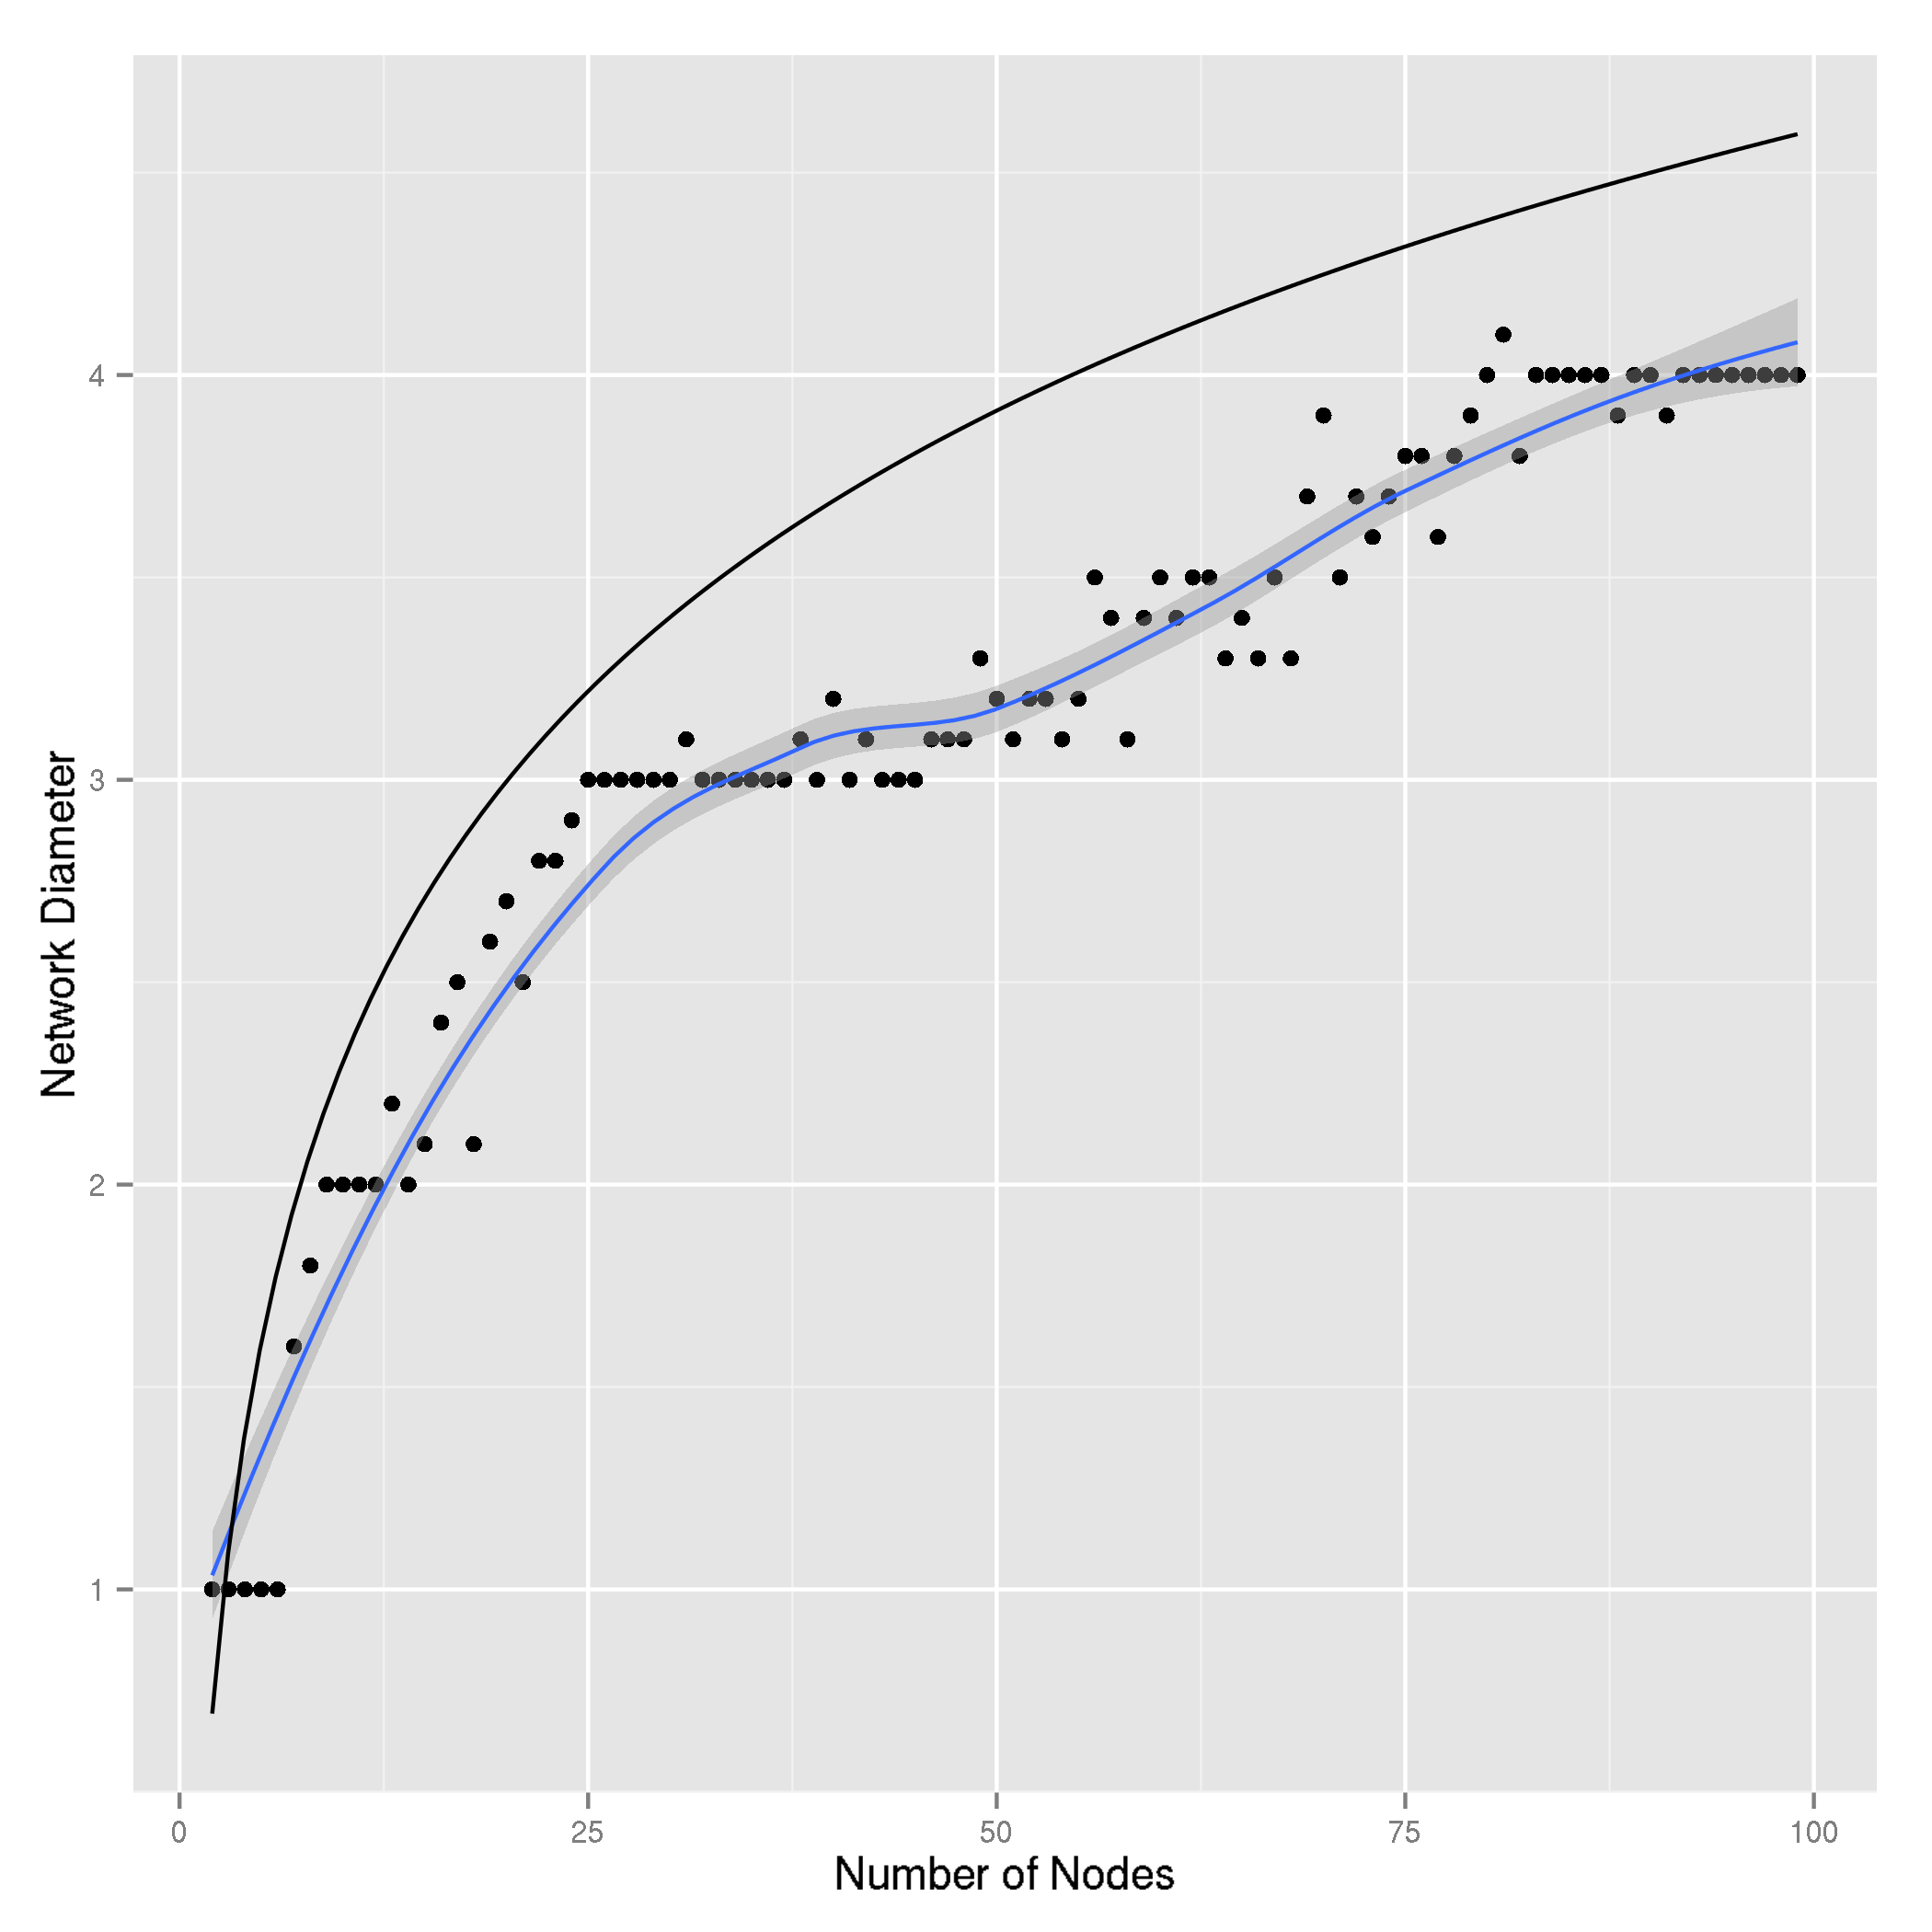
\includegraphics[scale=0.35]{./img/sizevsdiameter.png}
            \caption{Size vs.\ Diameter}
        \end{subfigure}
        \begin{subfigure}[b]{0.48\textwidth}
            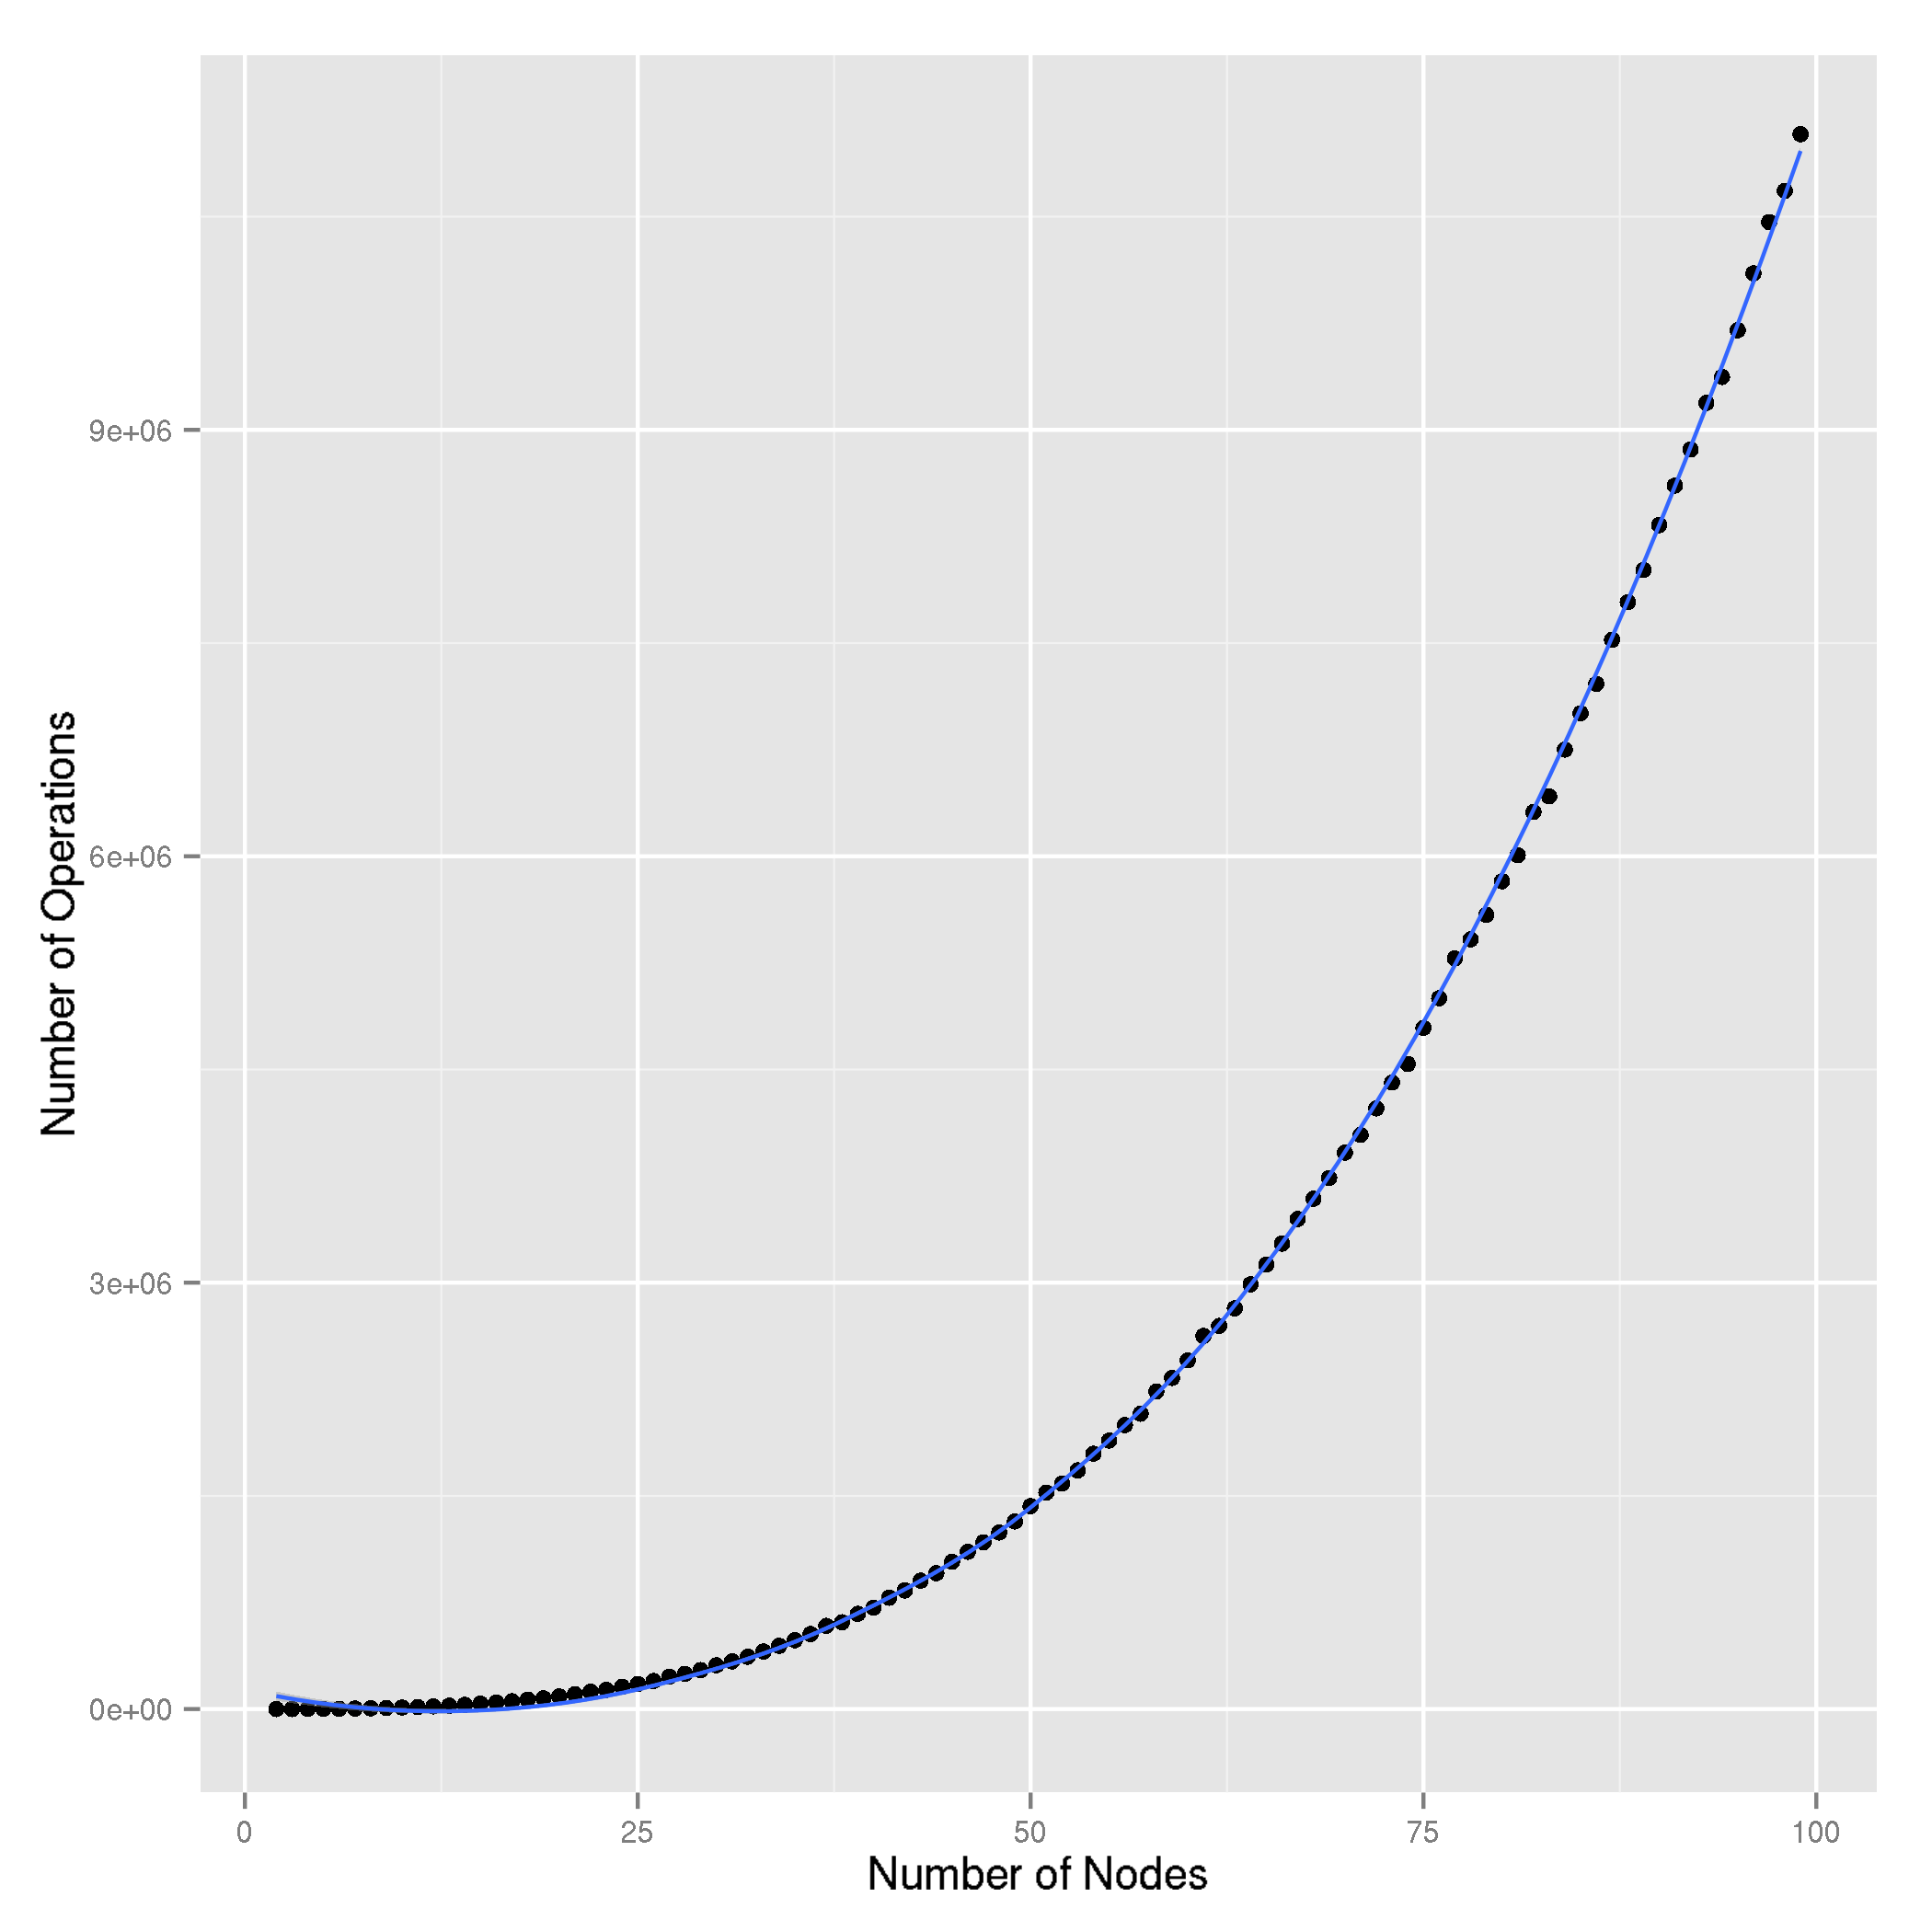
\includegraphics[scale=0.35]{./img/sizevsoperations.png}
            \caption{Size vs.\ Operations}
        \end{subfigure}

        \begin{subfigure}[b]{0.48\textwidth}
            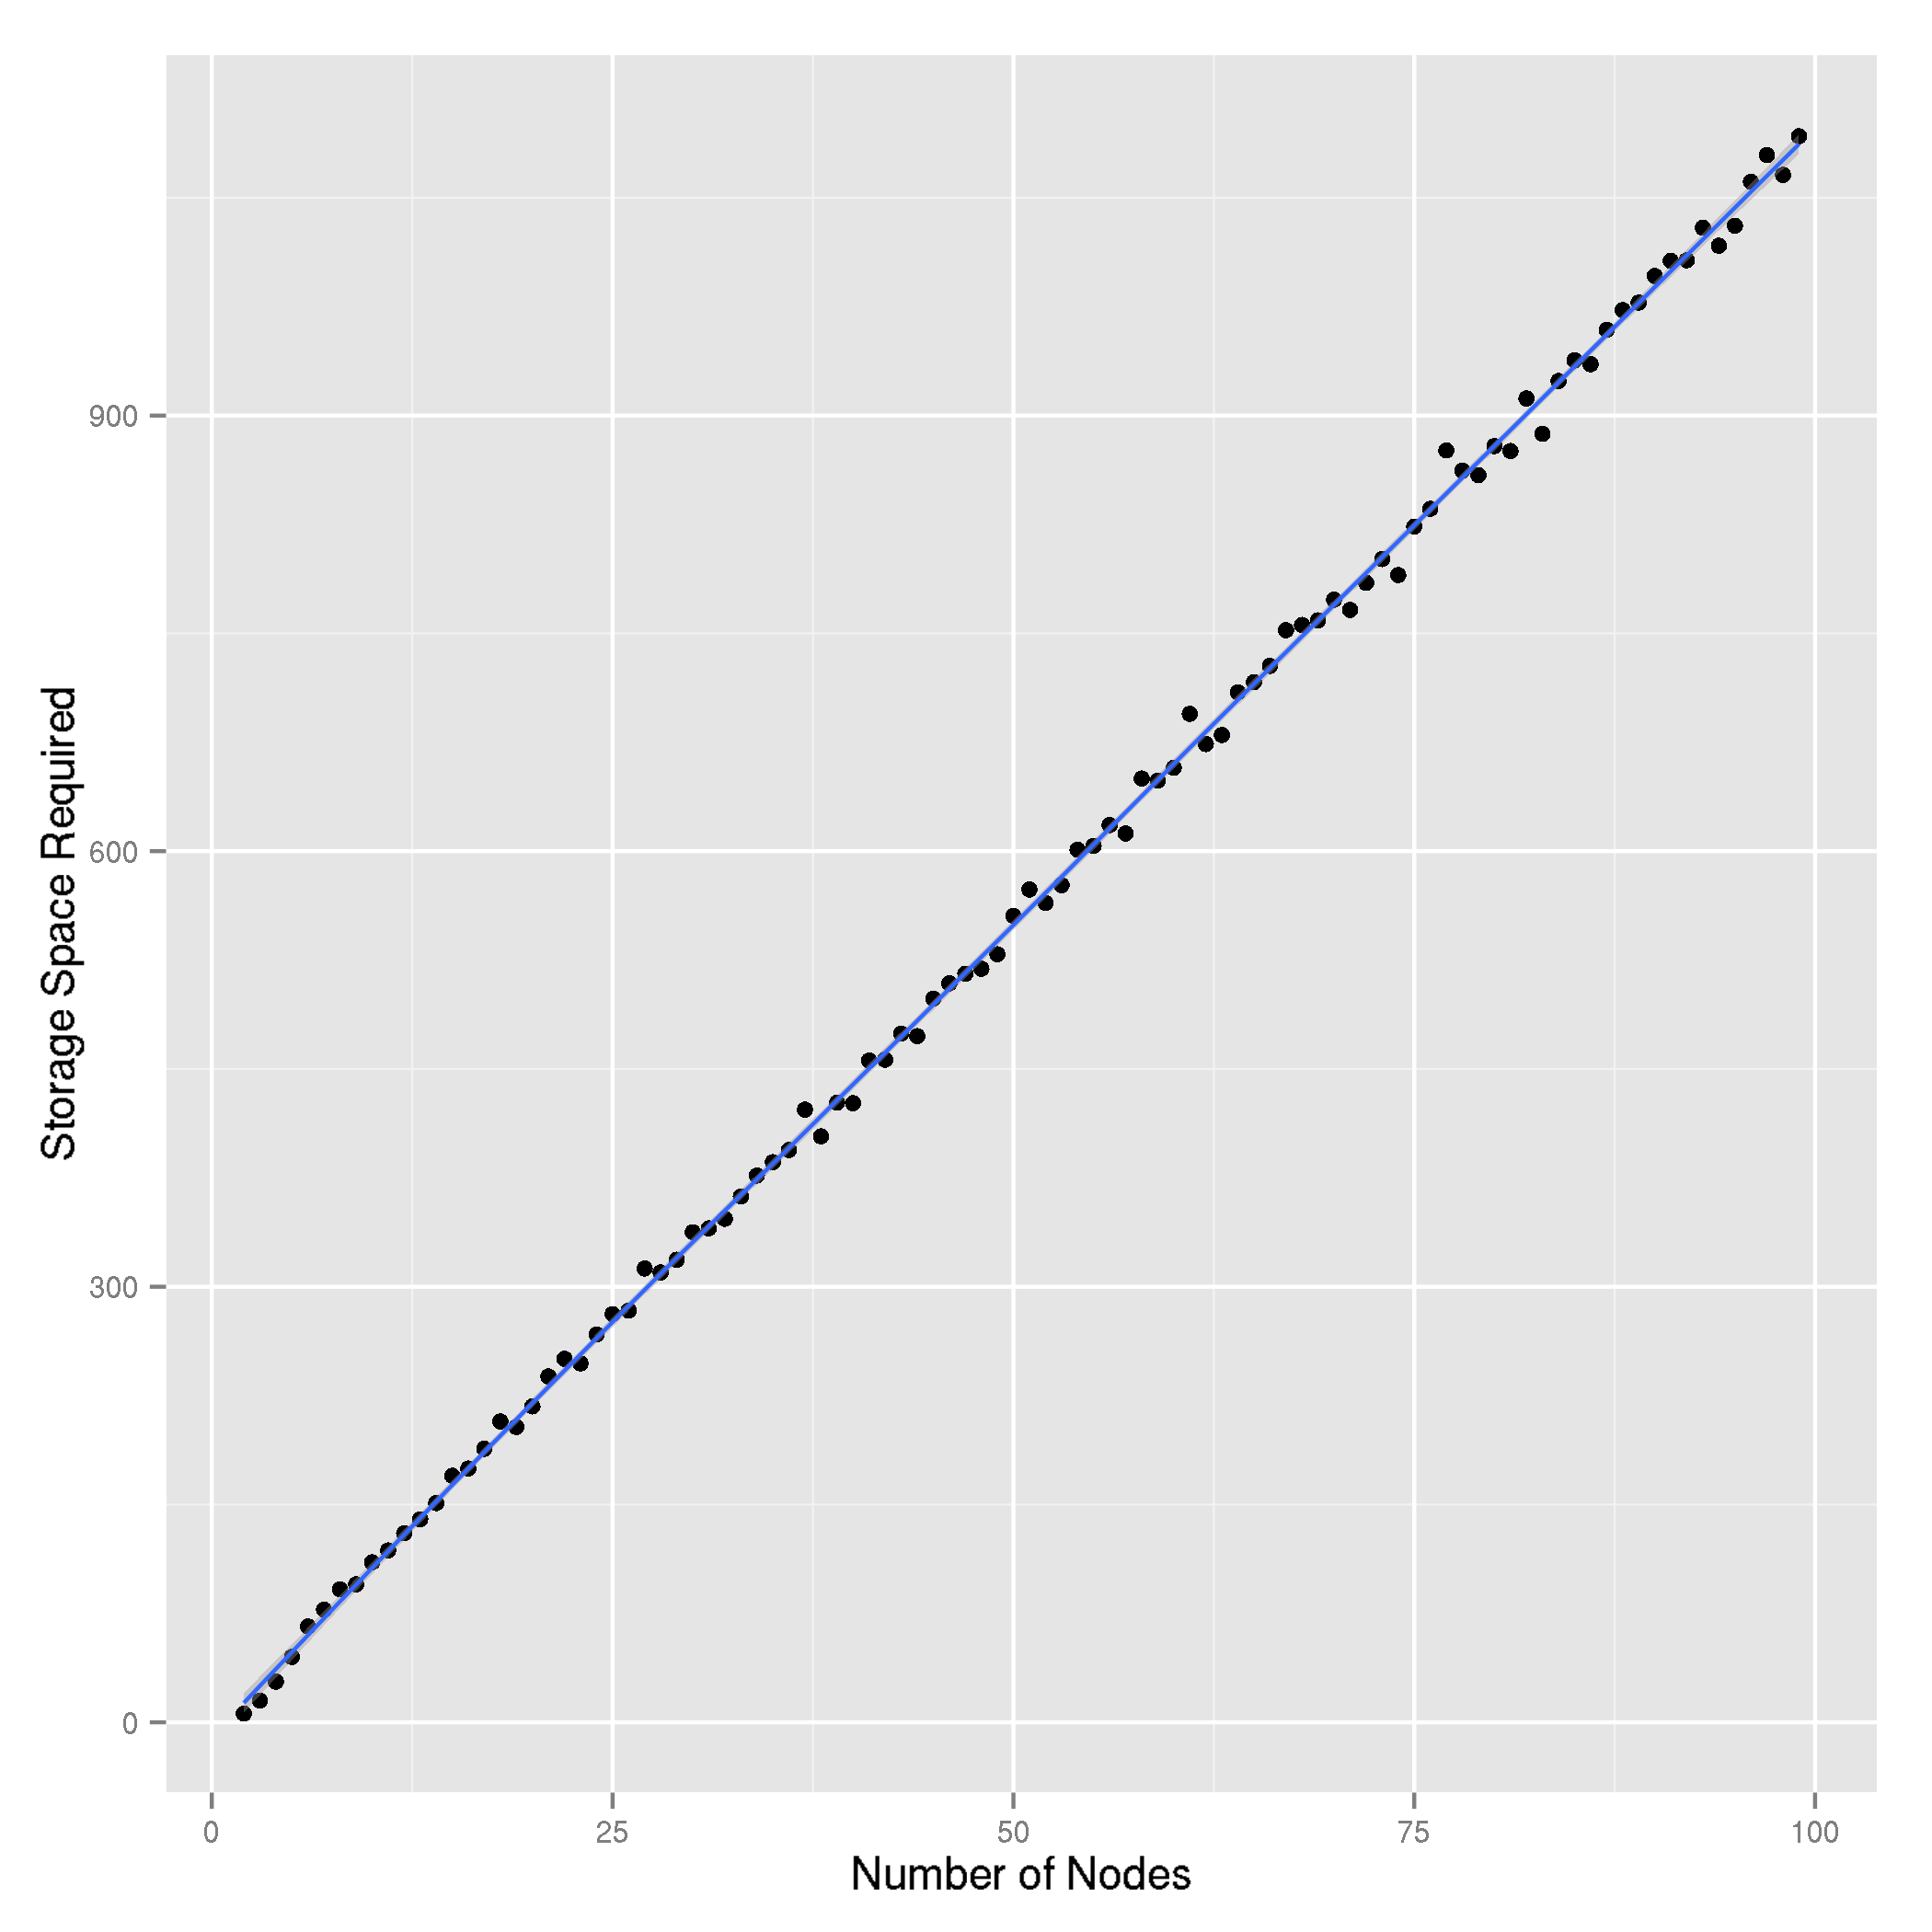
\includegraphics[scale=0.35]{./img/sizevsspace.png}
            \caption{Size vs.\ Space}
        \end{subfigure}
        \begin{subfigure}[b]{0.48\textwidth}
            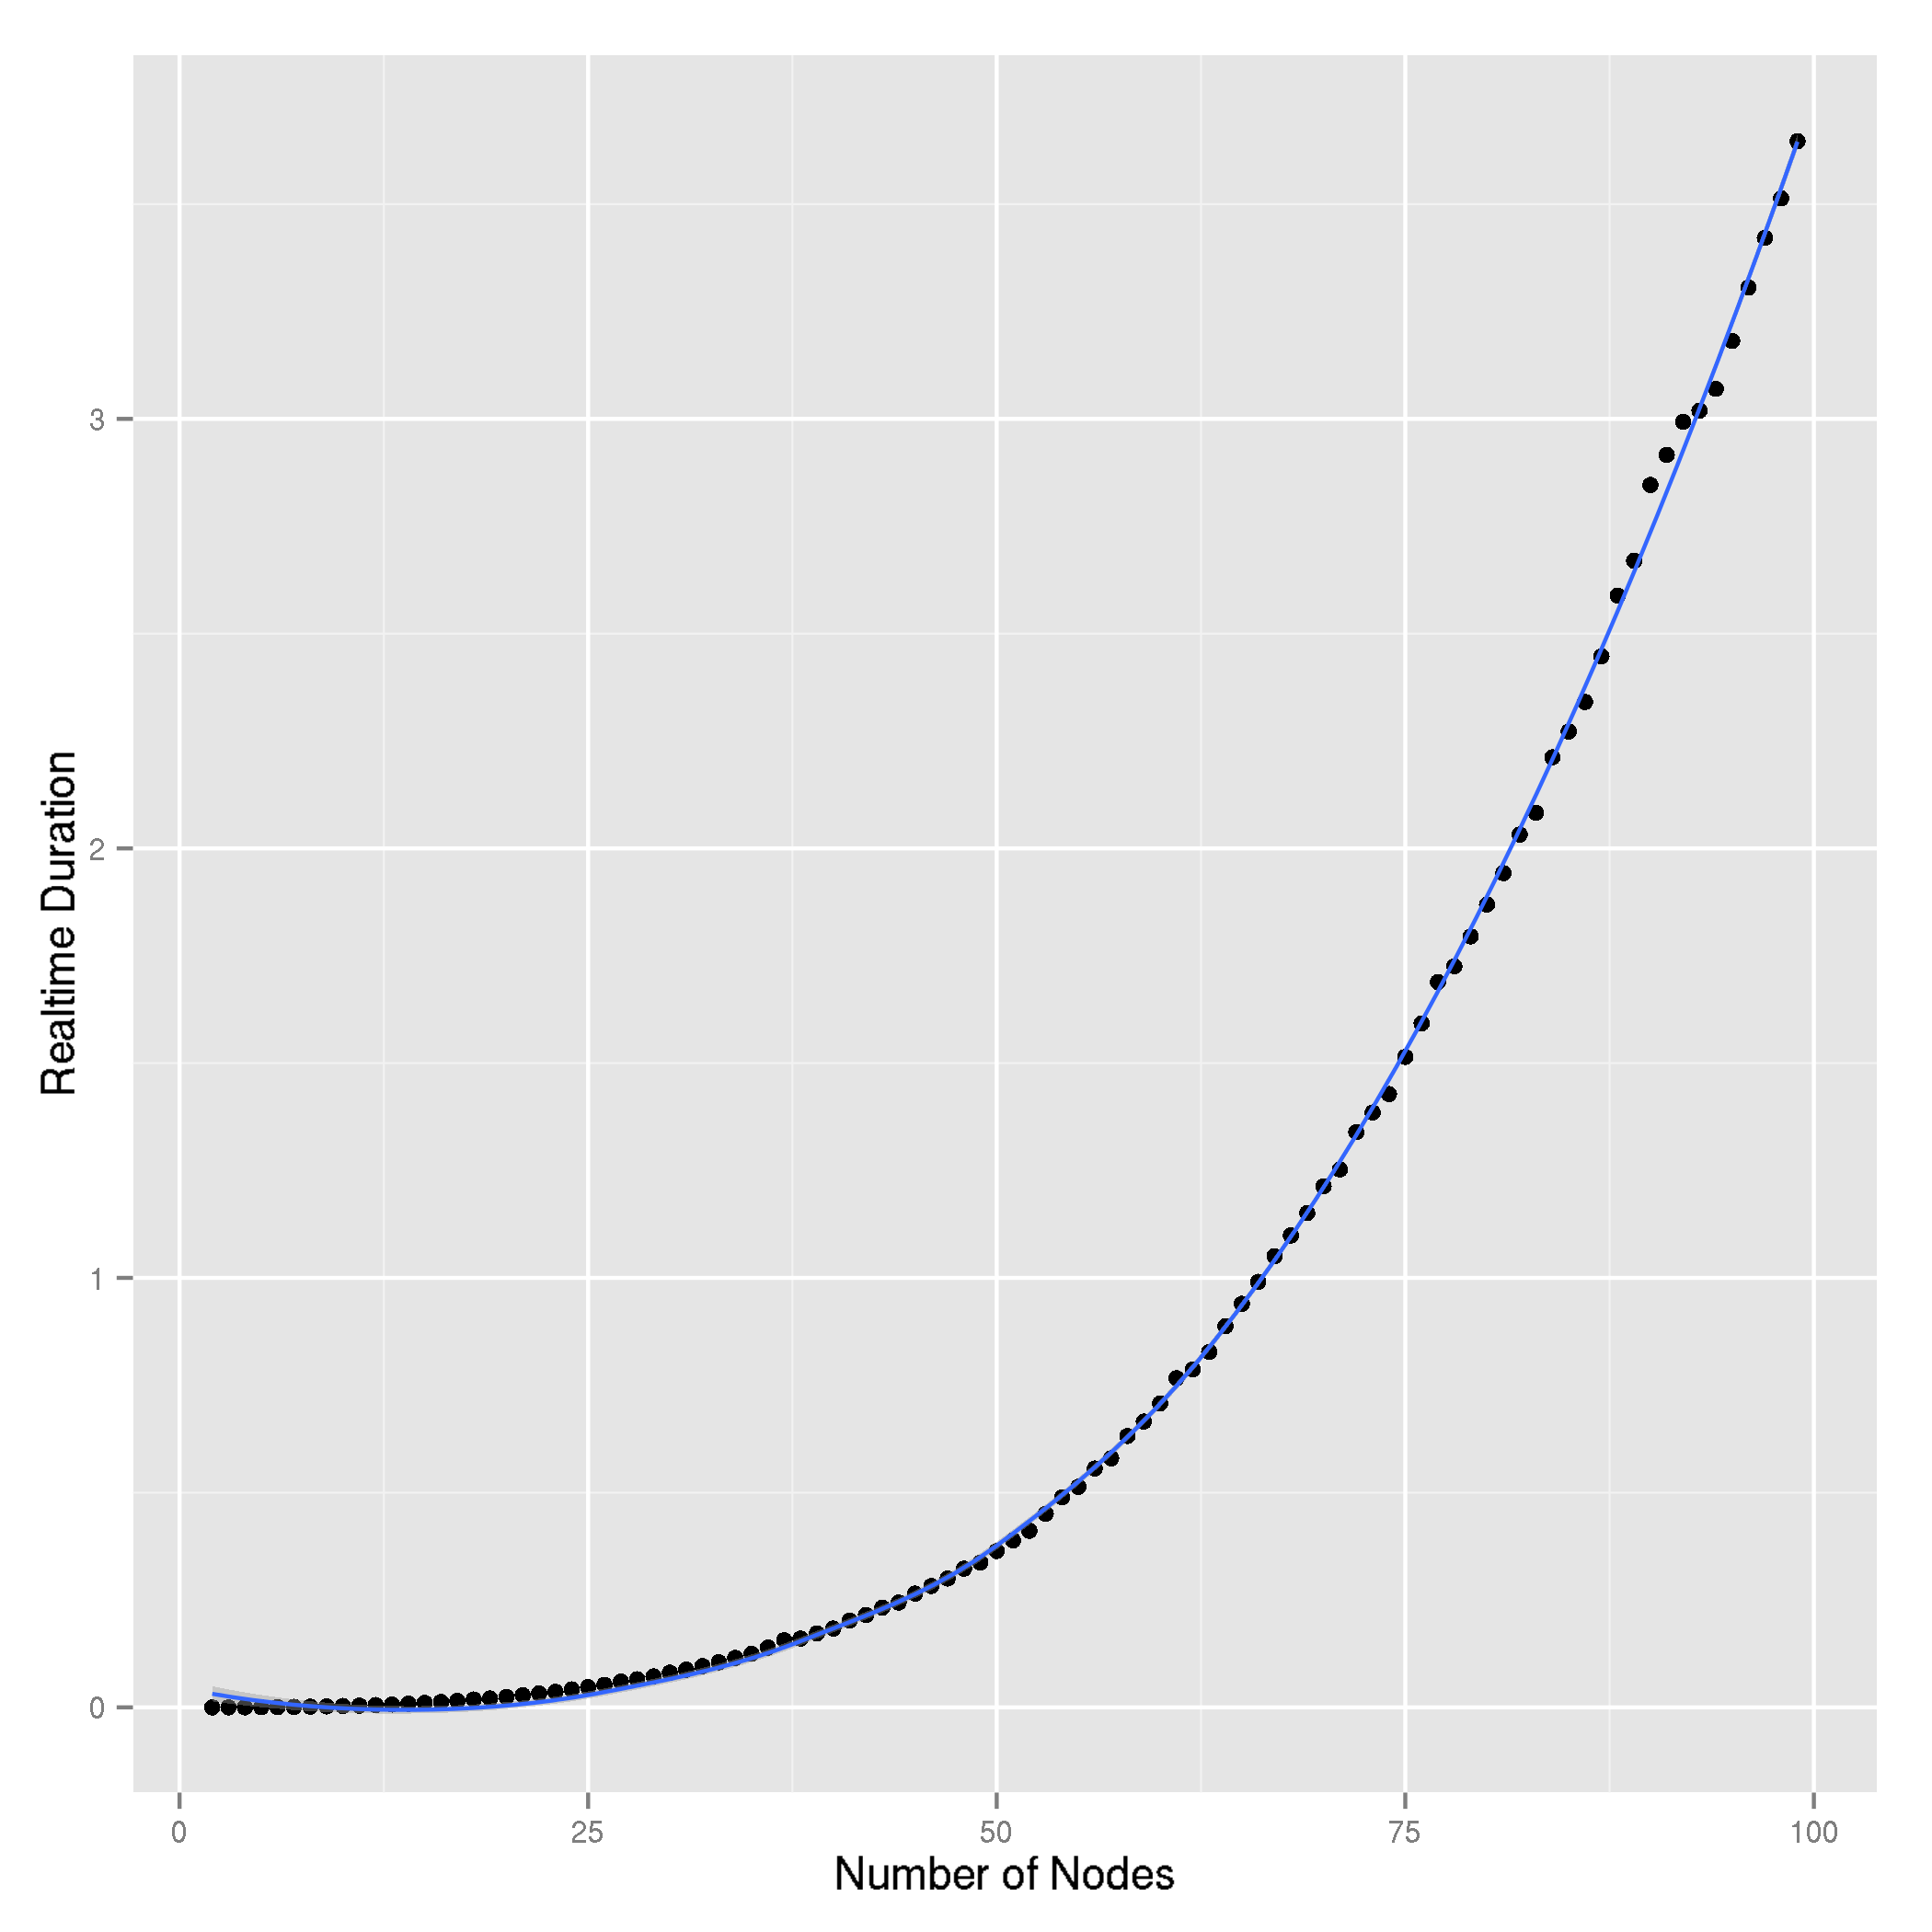
\includegraphics[scale=0.35]{./img/sizevstime.png}
            \caption{Size vs.\ Time}
        \end{subfigure}
        \caption{Diameter Estimation Analysis}
    \end{figure}

    @ Give an example of a directed graph $G = (V, E)$, a source vertex $s$ in $V$ and a set of tree edges $E_{\pi}
    \subset E$ such that for each vertex $v$ in $V$ , the unique path in the graph ($V, E_{\pi}$) from $s$ to $v$ is a
    shortest path in $G$, yet the set of edges $E_{\pi}$ cannot be produced by running a breadth-first search on $G$, no
    matter how the vertices are ordered in each adjacency list. Include a paragraph explaining why your example works.

    We have for example:

    \[
        \begin{aligned}
            V = \left[s, A, B, C, D\right]\\
            E = \left[(s, A), (s, B), (A, C), (A, D), (B, C), (B, D)\right]\\
            E = E_{\pi}\\
        \end{aligned}
    \]

    We see that in $E$, $A$ is before $B$. A Breadth-First-Search algorithm would push $(s, A)$ and $(s, B)$ onto the
    queue. Since a queue is First-In-Last-Out in Breadth-First-Search, $A$ will be loaded before $B$. This algorithm
    would then load $(A, C)$ and $(A, D)$, which would always be before $(B, C)$ and $(B, D)$, and $(A, D)$ and $(B, C)$
    would never be loaded together, Therefore, $E_{\pi}$ will never be produced. 
\end{easylist}

\end{document}
